The coincidence fraction $f$ at the optimal brightness threshold $n_{br,opt}$ is a measure for the binding fraction of the investigated sample. Its uncertainty $\sigma_f$ depends on the recorded number of bursts. For \gls{BTCCD}, an uncertainty lower than \SI{5}{\percent} is achievable \cite{Hoefig2019b}. Thus, the scope of the following measurement is to determine the required number of bursts to obtain an uncertainty lower than \SI{5}{\percent}.

\section{Measurement} \label{Section:OptimalNumberOfBursts_Measurement} 

A measurement of \SI{40}{\min} with dual-labeled \gls{dsDNA} was conducted by Olessya Yukhnovets (RWTH Aachen, Germany). Table~\ref{Table:Measurement_dlDNA_Olessya} includes information on the burst threshold, the background, and on the starting parameters.

\begin{table}[h]
	\centering
	\begin{tabular}{c|c|c|c|c|c} 
		ch. & $IPL^{thr}$ [\si{\micro\second}] & $\left\langle IPL^{bg} \right\rangle$ [\si{\micro\second}] & $\left\langle N \right\rangle$ [$10^{-3}$] & $\left\langle \tau_d \right\rangle$ [\si{\micro\second}] & $\left\langle MB \right\rangle$ [\si{\kilo\hertz}] \\
		\hline
		red & \num{150} & \num{1000} & \num{44.46 +- 0.33} & \num{1565.3 +- 9.6} & \num{27.8 +- 2.5} \\
		blue & \num{180} & \num{891} & \num{27.80 +- 0.18} & \num{1332.9 +- 5.8} & \num{22.7 +- 2.6} \\
	\end{tabular}
	\caption[Burst threshold, background, and starting parameters for measurement of dual-labeled \gls{dsDNA}, conducted by Olessya Yukhnovets (RWTH Aachen, Germany)]{Burst threshold, background, and starting parameters for a measurement of \SI{40}{\min} with dual-labeled \gls{dsDNA}.}
	\label{Table:Measurement_dlDNA_Olessya}
\end{table}

\section{Results and Discussion}

For the red channel, the coincidence fraction $f_{RB}$ at the optimal brightness threshold is given by
\begin{equation}
	f_{RB} (n_{br,opt}) = \frac{B_{RB}(n_{br,opt})}{B_R(n_{br,opt})},
\end{equation}
where $B_{RB}$ and $B_R$ denote the number of coincidence bursts, and the total number of selected bursts, respectively. According to Equation~\eqref{Equation:UncertaintyCoincidenceFractionRed}, the uncertainty $\sigma_{f_{RB}}$ is
\begin{equation}
	\sigma_{f_{RB}}(n_{br,opt}) = f_{RB}(n_{br,opt}) \sqrt{\frac{1}{B_R(n_{br,opt})} + \frac{1}{B_{RB}(n_{br,opt})}}.
\end{equation}
Substituting $B_{RB}(n_{br,opt}) = f_{RB}(n_{br,opt}) B_R(n_{br,opt})$, yields
\begin{equation} \label{Equation:UncertaintyCoincidenceFractionRedRewritten}
	\sigma_{f_{RB}}(n_{br,opt}) = \sqrt{\left(f_{RB}(n_{br,opt})\right)^2 + f_{RB}(n_{br,opt})} \cdot \frac{1}{\sqrt{B_R(n_{br,opt})}}.
\end{equation}
Thus, the uncertainty on $f_{RB}$ depends on the number of selected bursts. The pre-factor is determined by the coincidence fraction at the optimal brightness threshold, and takes values between \num{0} and $\sqrt{2}$. For the blue channel, the same equation is valid by substituting $RB \rightarrow BR$.

\clearpage

For a measurement of solely dual-labeled \gls{dsDNA}, a coincidence fraction of \SI{100}{\percent} is expected for both channels. Therefore, the pre-factor takes its highest possible value of $\sqrt{2}$. If an uncertainty of \SI{5}{\percent} is desired, the required minimum number of selected bursts for the red channel can be calculated by rearranging Equation~\eqref{Equation:UncertaintyCoincidenceFractionRedRewritten}
\begin{equation}
	B_R(n_{br,opt}) = \frac{2}{\left(\sigma_{f_{RB}}(n_{br,opt})\right)^2} = \frac{2}{0.05^2} = 800.
\end{equation}
For the blue channel, the same number is obtained.\\

Figure~\ref{fig:SelectedNumberOfBurstsRed} illustrates the dependency of the uncertainty on the selected bursts. The data points were obtained by splitting the \gls{IPL} time trace into several parts with increasing lengths. Each part contains an increasing number of bursts because of the corresponding increasing measurement time. For each part, the coincidence fraction and its uncertainty at the optimal brightness threshold is determined. The data follows Equation~\eqref{Equation:UncertaintyCoincidenceFractionRedRewritten}. For approximately $B_R(n_{br,opt}) = 800$, the uncertainty falls below \SI{5}{\percent}. For the blue channel, a similar behavior is observed, see Figure~\ref{fig:SelectedNumberOfBurstsBlue}. There, the uncertainty drops below \SI{5}{\percent} slightly before $B_B(n_{br,opt}) = 800$ because the experimentally determined coincidence fraction is not exactly \SI{100}{\percent} but slightly lower. Thus, the pre-factor of Equation~\eqref{Equation:UncertaintyCoincidenceFractionRedRewritten} is a bit smaller.

\begin{figure}[h]
	\centering
	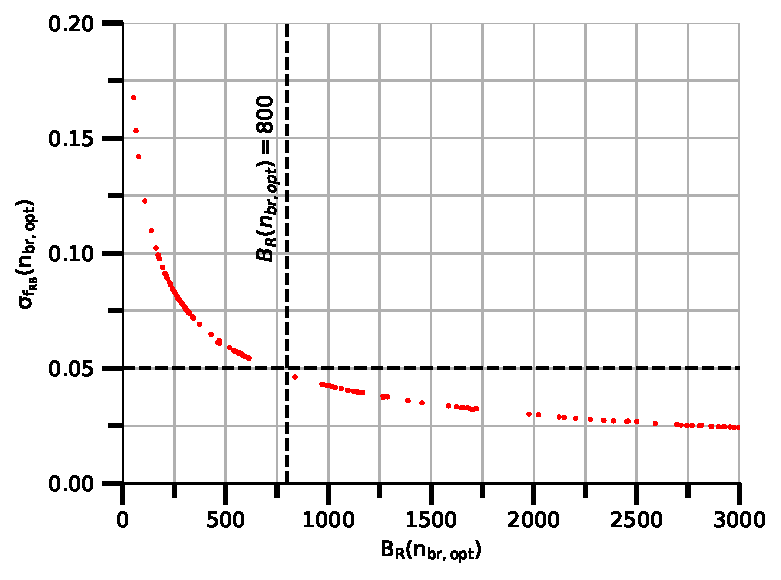
\includegraphics[width=4in]{OptimalNumberOfSelectedBurstsRed.pdf}
	\caption[Optimal number of selected bursts for red channel]{Uncertainty on the coincidence fraction $f_{RB}$ at the optimal brightness threshold $n_{br,opt}$ as a function of the selected number of bursts $B_R(n_{br,opt})$ for the red channel. The optimal number of selected bursts, for which the uncertainty falls below \SI{5}{\percent}, is approximately $B_R(n_{br,opt}) = 800$.}
	\label{fig:SelectedNumberOfBurstsRed}
\end{figure} 

The pre-factor and thus the uncertainty take their largest values for a coincidence fraction of \SI{100}{\percent}. If the expected coincidence fraction for a measurement is lower, the pre-factor can be adjusted. Nonetheless, it has to be paid attention to chance coincidences that increase the coincidence fraction $f_{RB}$. The effect of chance coincidences on the coincidence fraction is further discussed in Chapter~\ref{Chapter:ChanceCoincidenceLimitation}.\\

Another way to illustrate the uncertainty on the coincidence fraction at the optimal brightness threshold is a plot against the initial number of bursts $B_R(0)$. The advantage is that this number is known before the application of \gls{BTCCD}, and can be used to estimate the required measurement time. Figure~\ref{fig:TotalNumberOfBurstsRed} illustrates such a plot for the red channel. The initial number of bursts $B_R(0)$ does not determine the uncertainty completely because $\sigma_{f_{RB}}(n_{br,opt})$ depends only on the selected number of bursts $B_R(n_{br,opt})$. $B_R(0)$ and $B_R(n_{br,opt})$ are correlated as more initial bursts include most likely more selected bursts, but there is no deterministic relationship. Nonetheless, it can be seen that, for around \num{10000} initial bursts, the uncertainty is most probably lower than \SI{5}{\percent}. For the blue channel, even around \num{7500} initial bursts are sufficient, see Figure~\ref{fig:TotalNumberOfBurstsBlue}.

\begin{figure}[h]
	\centering
	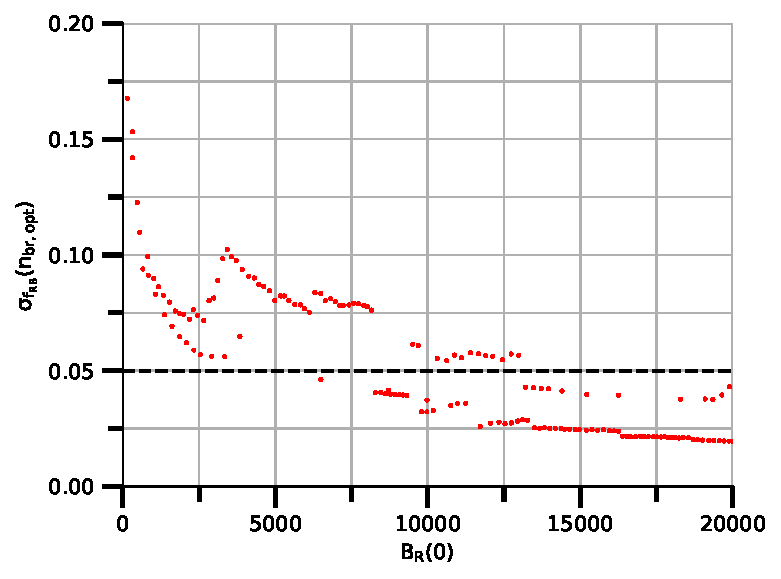
\includegraphics[width=4in]{OptimalNumberOfTotalBurstsRed.pdf}
	\caption[Optimal number of initial bursts for red channel]{Uncertainty on the coincidence fraction $f_{RB}$ at the optimal brightness threshold $n_{br,opt}$ as a function of the initial number of bursts $B_R(0)$ for the red channel. The graph does not reveal a completely deterministic behavior. However, for a number of about \num{10000} initial bursts, the uncertainty is typically lower than \SI{5}{\percent}.}
	\label{fig:TotalNumberOfBurstsRed}
\end{figure} 

To sum it up, the uncertainty at the optimal brightness threshold depends on the value of the coincidence fraction. If the coincidence fraction is almost \SI{100}{\percent}, \num{800} selected bursts for both channels are sufficient to obtain an uncertainty of less than \SI{5}{\percent}. There is no strict relation between the uncertainty and the initial number of bursts. Nonetheless, about \num{10000} initial bursts lead most likely to an uncertainty below \SI{5}{\percent}. For smaller coincidence fractions, the required number of bursts becomes less. Hence, \num{10000} recorded initial bursts, or \num{800} selected bursts guarantee an uncertainty of less than \SI{5}{\percent} for both channels.